% Copyright 2004 by Till Tantau <tantau@users.sourceforge.net>.
%
% In principle, this file can be redistributed and/or modified under
% the terms of the GNU Public License, version 2.
%
% However, this file is supposed to be a template to be modified
% for your own needs. For this reason, if you use this file as a
% template and not specifically distribute it as part of a another
% package/program, I grant the extra permission to freely copy and
% modify this file as you see fit and even to delete this copyright
% notice. 

%\documentclass[pdftex,12pt]{article}	% the pdftex is essential

\documentclass[pdftex]{beamer}
\usepackage{graphicx}            % to include images
%\usepackage{pslatex}	    % to use PostScript fonts
\usepackage{amsmath} 
%\usepackage[margin=1.25in]{geometry}
\usepackage{textcomp}
\usepackage{courier}
\usepackage{gensymb} %has degree symbol
%\usepackage{times}
\usepackage [english]{babel}
\usepackage [autostyle, english = american]{csquotes}
%\usepackage{cite}
\MakeOuterQuote{"}
%\usepackage{fancyhdr} %fancy page numbers
%\usepackage{lastpage} %get the last page number
%\usepackage[doublespacing]{setspace}
%\usepackage{multirow}

\usepackage[maxbibnames=99, defernumbers, style=nejm]{biblatex}
\addbibresource{smartutilities.bib} 

% There are many different themes available for Beamer. A comprehensive
% list with examples is given here:
% http://deic.uab.es/~iblanes/beamer_gallery/index_by_theme.html
% You can uncomment the themes below if you would like to use a different
% one:
%\usetheme{AnnArbor}
%\usetheme{Antibes}
%\usetheme{Bergen}
%\usetheme{Berkeley}
%\usetheme{Berlin}
%\usetheme{Boadilla}
%\usetheme{boxes}
\usetheme{CambridgeUS}
%\usetheme{Copenhagen}
%\usetheme{Darmstadt}
%\usetheme{default}
%\usetheme{Frankfurt}
%\usetheme{Goettingen}
%\usetheme{Hannover}
%\usetheme{Ilmenau}
%\usetheme{JuanLesPins}
%\usetheme{Luebeck}
%\usetheme{Madrid}
%\usetheme{Malmoe}
%\usetheme{Marburg}
%\usetheme{Montpellier}
%\usetheme{PaloAlto}
%\usetheme{Pittsburgh}
%\usetheme{Rochester}
%\usetheme{Singapore}
%\usetheme{Szeged}
%\usetheme{Warsaw}
\usecolortheme{dolphin}
%\usetheme{Warsaw}
\usefonttheme{"structurebold"}

\title[Continuous snSMARTs]{Small Sample Sequential Multiple Assignment Randomized Trials with Continuous Repeated Measures}
\subtitle{ENAR 2020}

% A subtitle is optional and this may be deleted


\author{Holly Hartman}
% - Give the names in the same order as the appear in the paper.
% - Use the \inst{?} command only if the authors have different
%   affiliation.

\institute[]{\normalsize
Roy Tamura, Matthew Schipper, Kelley Kidwell \\ [\baselineskip]
 holhart@umich.edu \\
https://holly-hartman.com \\
@holly7holly
}


\date{March 25, 2020}
% If you have a file called "university-logo-filename.xxx", where xxx
% is a graphic format that can be processed by latex or pdflatex,
% resp., then you can add a logo as follows:

% \pgfdeclareimage[height=0.5cm]{university-logo}{university-logo-filename}
% \logo{\pgfuseimage{university-logo}}

%\setbeamertemplate{footline}[frame number]
\usenavigationsymbolstemplate{}

% Let's get started
\begin{document}

\begin{frame}
  \titlepage
\end{frame}

% Section and subsections will appear in the presentation overview
% and table of contents.

%%\subsection{Overview}


\begin{frame}{snSMART Goals}
\begin{itemize}

\item snSMARTs designs can be used to more efficiently identify the best treatment overall and use Bayesian methods [\cite{Huo2017, Wei2018}].
\item Both require dichotomous determination of "response" to determine the second stage treatment (sometimes called a tailoring variable) [\cite{Lei2012, Amirall2012}].
\end{itemize}
\end{frame}

\begin{frame}{snSMART  Design}
\begin{center}
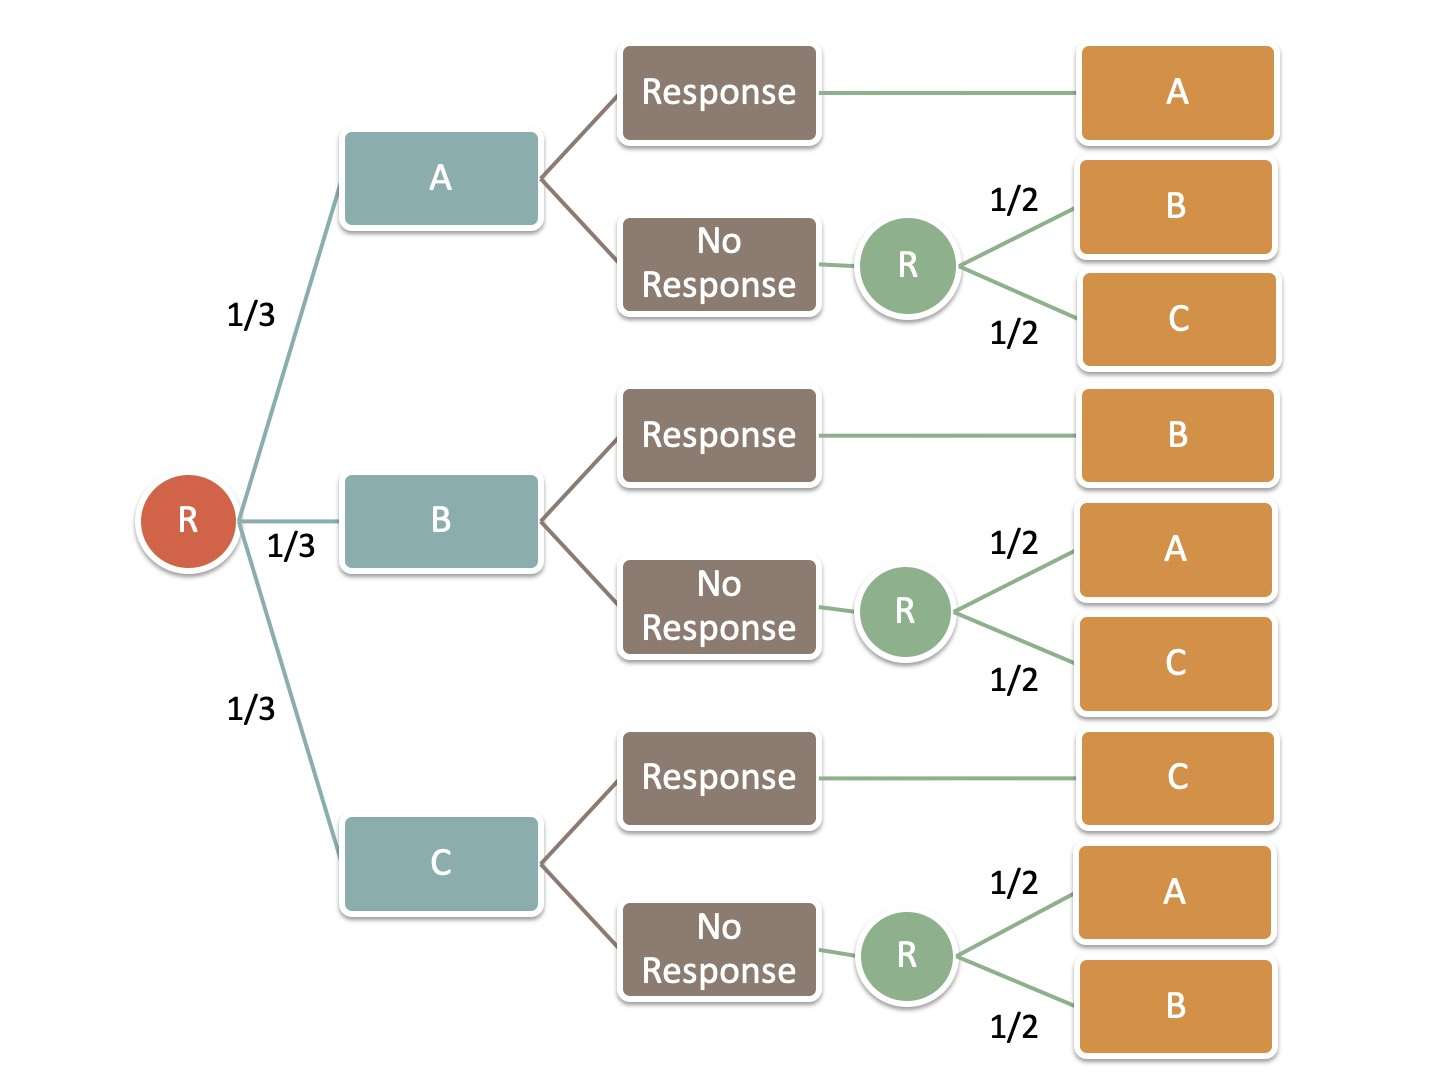
\includegraphics[scale=.2]{snsmart.jpg}
\end{center}
\end{frame}


\begin{frame}{Problems with binary outcomes}
\begin{itemize}
\item In rare diseases or other areas with little prior knowledge, a clear choice for a dichotomization method or a binary surrogate may not be available prior to the start of the study.
\item Pilot studies can be expensive and cost prohibitive.
\item If a dichotomized continuous variable is used as outcome, can result in loss of statistical power [\cite{Snapinn2007}].
\end{itemize}
\end{frame}

\begin{frame}{Continuous snSMART Design}
\begin{center}
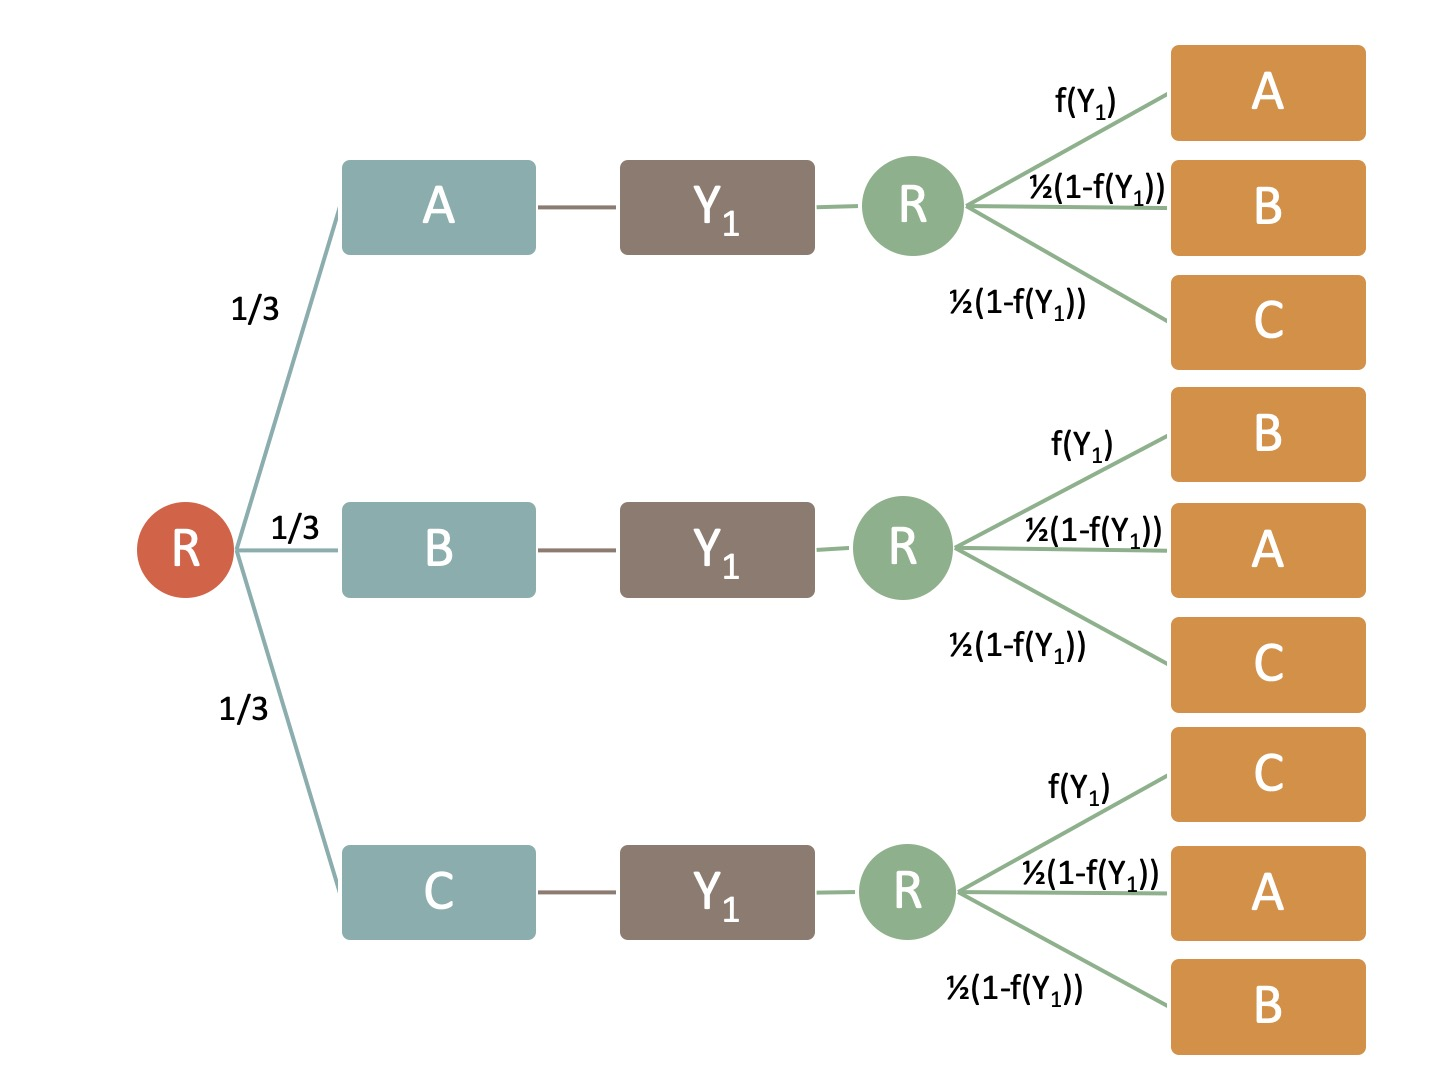
\includegraphics[scale=.2]{csnsmart.jpg}
\end{center}
\end{frame}


\begin{frame}{snSMART design with continuous repeated measures}

\begin{itemize}
\item Goal: identify the best treatment at the end of the first stage.
\item Use a mapping function to map first stage outcome $Y_{i1}$ to $\left[0,1\right]$ and is the probability of staying on the same treatment.
\item Better outcomes of $Y_{i1}$ should map to values closer to 1
\item Options for the Mapping Function:
\begin{itemize}
\item Linear function between minimum and maximum values of $Y_1$
\begin{itemize}
\item $f(Y_1) = (Y_1- Y_{min})/(Y_{max} - Y_{min})$
\item Can also modify with powers, $f(Y_1)^k$, if distribution is expected to be skewed or it would be beneficial to have more/fewer people stay on the treatment 
\end{itemize}
\item Function between practical/ethical values of $Y_1$ and 0 or 1 beyond these limits
\end{itemize}
\end{itemize}
\end{frame}


\begin{frame}{Models}
Goal (mathematically): Estimate all $\beta_j$ parameters (treatment effects at the end of the first stage).\\
Mean Model:\\

$$\mu_1(T_{i1}) = \sum_{j=1}^T \beta_j I(T_{i1} = j) $$
$$\mu_2 (T_{i1}, T_{i2})  = \alpha_1 \sum_{j=1}^T \beta_{j} I(T_{i1} = j) + \alpha_2 \sum_{k=1}^T \beta_{k} I(T_{i2} = k) + \alpha_3I(T_{i1}=T_{i2}) $$ 

Covariance Model:\\
$$\mathbf{V}(T_{i1}, T_{i,2}) = V_1 I(T_{i1} = T_{i2}) + V_2  I(T_{i1} \neq T_{i2}) $$  
where $V_1$ and $V_2$ are both $2 \times 2$ variance-covariance matrices.
\end{frame}


\begin{frame}{Priors}
\begin{center}
\begin{tabular}{ll}
$\beta_j \sim  N( \text{mean} = 50, \text{standard deviation (sd) = }50) $ for all $j$ \\
$\alpha_1 \sim Unif(0,0.5)$ &  \\
$\alpha_3 \sim FN(\text{mean = }0, \text{sd} = 20)$\\
$V_1 \sim W_2\left( \begin{bmatrix}
1 & 0 \\
0 & 1
\end{bmatrix}, 2 \right)$ & \\
$V_2 \sim W_2\left( \begin{bmatrix}
1 & 0 \\
0 & 1
\end{bmatrix}, 2 \right)$ &  \\
\end{tabular}\\
\end{center}
\vspace{1em}
These priors impose 3 conditions for the $\alpha$ parameters:\\
1) $\alpha_2 =  1- \alpha_1$ \\
 2) $\alpha_2 > \alpha_1$ \\
 3) $\alpha_3 \ge 0$
\end{frame}

\begin{frame}{Ideal scenarios}
\begin{itemize}
\item $\alpha = (0.2, 0.8, 5)$
\end{itemize}
$$ V_1 = \sigma^2
 \begin{bmatrix} 1 & \tau_1 \\
 \tau_1 & 1 \end{bmatrix},  V_2 = \sigma^2
 \begin{bmatrix} 1 & \tau_2 \\
 \tau_2 & 1 \end{bmatrix}
$$
\begin{itemize}
\item $\tau_1 = 0.8$, $\tau_2 = 0.3$, and $\sigma = 20$
\end{itemize}
\begin{center}
\begin{tabular}{c|ccc}\hline
& \multicolumn{3}{c}{$\beta$}  \\ \hline 
Scenario & 1 & 2 & 3  \\ \hline
1 & 40 & 50 & 60   \\
2 & 20 & 30 & 40  \\
3 & 60 & 70 & 80  \\ \hline
\end{tabular}
\end{center}
\end{frame}

\begin{frame}{Scenarios with model assumption violations}
\begin{itemize}
\item We examined 3 assumption violations
\begin{itemize}
\item Second stage treatment effect, $\mu_2$, is based on the treatment specific pathway (TSP) rather than weighted means
\item Variance, $\sigma^2$, varies depending on treatment
\item Correlation, $\tau$, depends on the TSP (treatments may have more or less correlation based on treatment mechanism similarities)
\end{itemize}
\item All other parameters were the same as scenario 1.
\end{itemize}
\end{frame}

\begin{frame}{Scenarios}
\begin{center}
\begin{tabular}{c|ccc|ccc}\hline
& \multicolumn{3}{c|}{$\beta$} & \multicolumn{3}{c}{Violation} \\ \hline 
Scenario & 1 & 2 & 3 & Mean & Variance & Correlation  \\ \hline
1 & 40 & 50 & 60 & &  &  \\
2 & 20 & 30 & 40 & &  &  \\
3 & 60 & 70 & 80 &  &  &  \\ 
4 & 40 & 50 & 60 & $\times$ & & \\
5 & 40 & 50 & 60 & & $\times$ & \\
6 & 40 & 50 & 60 & & & $\times$ \\
7 & 40 & 50 & 60 & $\times$ & $\times$ & \\
8 & 40 & 50 & 60 & $\times$ & & $\times$ \\
9 & 40 & 50 & 60 & & $\times$ & $\times$ \\
10 & 40 & 50 & 60 & $\times$ & $\times$ & $\times$\\ \hline
\end{tabular}
\end{center}
\end{frame}

\begin{frame}{Mapping functions}
\begin{itemize}
\item Used 3 mapping functions
\begin{itemize}
\item $MF 1 =  Y_1/100$
\item $MF 2 = (Y_1/100)^2$
\item $MF 1/2= (Y_1/100)^{1/2}$
\end{itemize}
\item For scenarios 1, 2, and 3 compared to dichotomized outcomes (DO) using dichotomization of the continuous first stage outcome with 3 different cut offs:
\begin{itemize}
\item DO 30 = 30
\item DO 50 = 50
\item DO 70 = 70
\end{itemize}
\end{itemize}
\end{frame}


\begin{frame}{Results for ideal scenarios}
\begin{center}
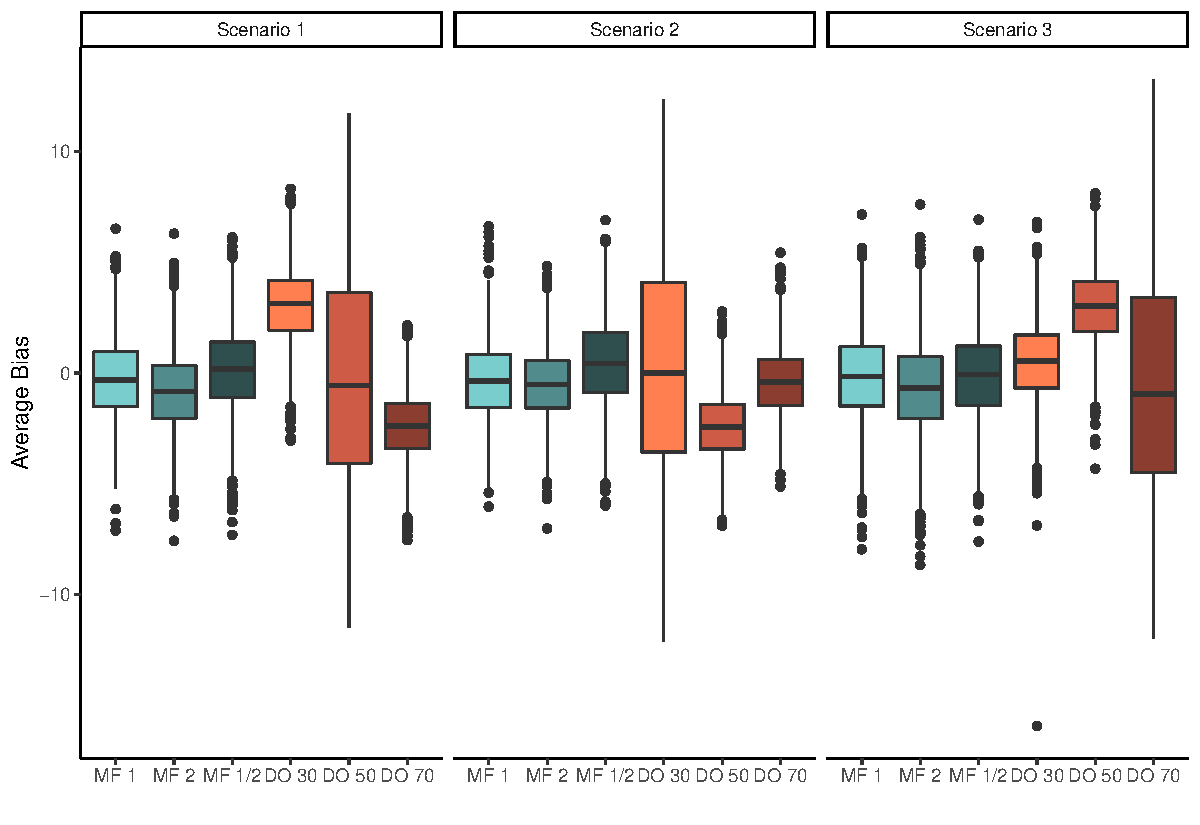
\includegraphics[scale=.5]{idealscen.pdf}
\end{center}
\end{frame}

\begin{frame}{Results for model assumption violations}
\begin{center}
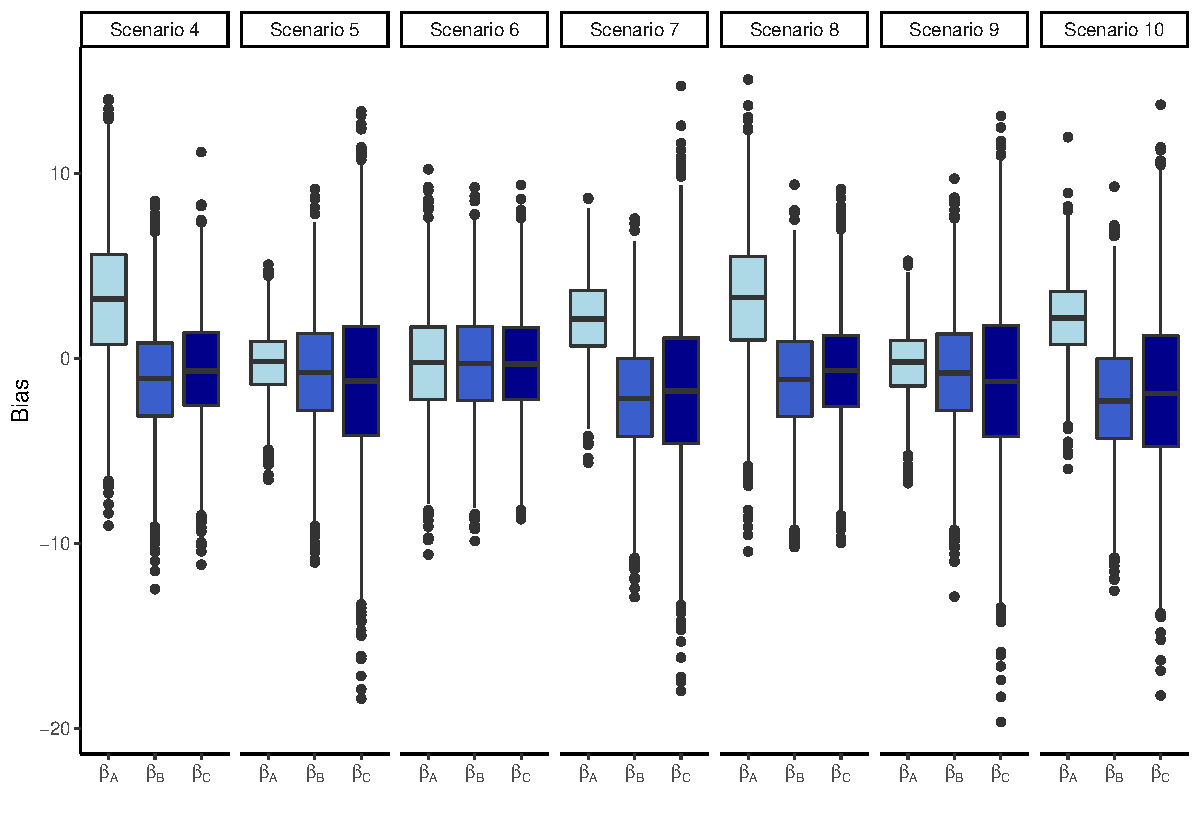
\includegraphics[scale=.5]{assumpviol.pdf}
\end{center}
\end{frame}


\begin{frame}{Patient outcomes}
\begin{center}
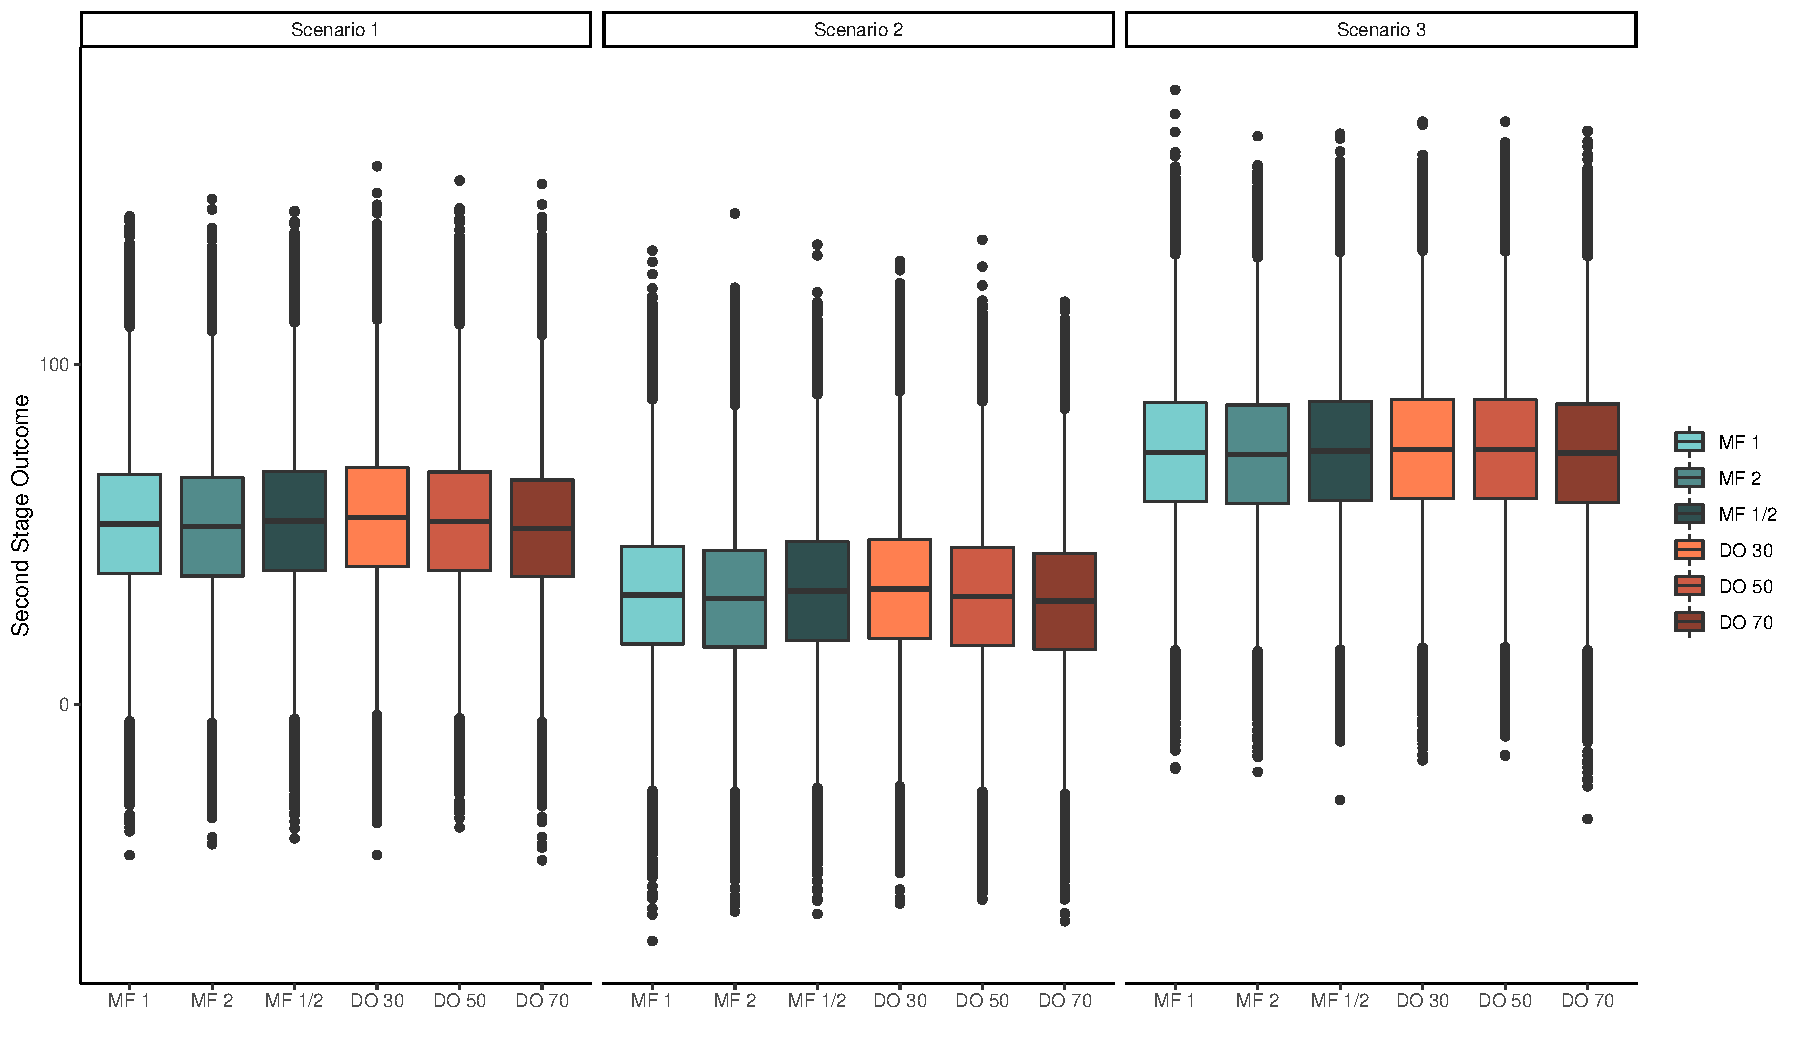
\includegraphics[scale=.4]{outFinalColor.pdf}
\end{center}
\end{frame}

\begin{frame}{Conclusions}
\begin{itemize}
\item Mapping functions are a reasonable method for conducting a snSMART design in the absence of a binary variable.
\item Patient outcomes are similar to when using a dichotomous outcome.
\item Using a mapping function improves the number of treatment pathways seen in a trial relative to a poorly selected dichotomous outcome. 
\end{itemize}
\end{frame}


\begin{frame}{References}
\AtNextBibliography{\footnotesize}
\printbibliography

\end{frame}

%\begin{frame}{References}
%\bibliography{library}{}
%\bibliographystyle{plain}
%\end{frame}

\end{document}

